%
% File acl2015.tex
%
% Contact: car@ir.hit.edu.cn, gdzhou@suda.edu.cn
%%
%% Based on the style files for ACL-2014, which were, in turn,
%% Based on the style files for ACL-2013, which were, in turn,
%% Based on the style files for ACL-2012, which were, in turn,
%% based on the style files for ACL-2011, which were, in turn, 
%% based on the style files for ACL-2010, which were, in turn, 
%% based on the style files for ACL-IJCNLP-2009, which were, in turn,
%% based on the style files for EACL-2009 and IJCNLP-2008...

%% Based on the style files for EACL 2006 by 
%%e.agirre@ehu.es or Sergi.Balari@uab.es
%% and that of ACL 08 by Joakim Nivre and Noah Smith

\documentclass[11pt]{article}
\usepackage{acl2015}
\usepackage{times}
\usepackage{url}
\usepackage{latexsym}
\usepackage{graphicx}
\usepackage{amsmath}

%\setlength\titlebox{5cm}

% You can expand the titlebox if you need extra space
% to show all the authors. Please do not make the titlebox
% smaller than 5cm (the original size); we will check this
% in the camera-ready version and ask you to change it back.


\title{CS224n PA1}

\author{Justin Cunningham \\
  {\tt jcnnghm@stanford.edu}}

\date{October 6, 2015}

\DeclareMathOperator*{\argmax}{arg\,max}

\begin{document}
\maketitle
\begin{abstract}
  In programming assignment 1, I implemented a pointwise mutual
  information (PMI) word aligner, as well as IBM Model 1 and
  IBM Model 2 word aligners.  The PMI Aligner achieved an AER of
  0.6837, while Model 1 and Model 2 achieved 0.4314
  and 0.3775 respectively.  In the second part of the assignment,
  I implemented a feature for Phrasal which was able to achieve a
  15.761 average BLEU score.
\end{abstract}

\section{Part 1}

\begin{table*}
  \begin{center}
    \begin{tabular}{ l c c c }
      \hline
      & French-English & Hindi-English & Chinese-English \\
      \hline
      PMI     & 0.6837 & 0.8376 & 0.8444 \\
      Model 1 & 0.4314 & 0.5838 & 0.6534 \\
      Model 2 & 0.3775 & 0.5901 & 0.6238 \\
      \hline
    \end{tabular}
  \end{center}
  \caption{AER results for development set.}
  \label{table:dev}
\end{table*}

\begin{table*}
  \begin{center}
    \begin{tabular}{ l c c c }
      \hline
      & French-English & Hindi-English & Chinese-English \\
      \hline
      PMI     & 0.6215 & 0.8309 & 0.8519 \\
      Model 1 & 0.3994 & 0.5473 & 0.6559 \\
      Model 2 & 0.3265 & 0.5651 & 0.6435 \\
      \hline
    \end{tabular}
  \end{center}
  \caption{AER results for test set.}
  \label{table:test}
\end{table*}

In Part 1, I implemented PMI and IBM Model 1 and IBM Model 2.
AER results for all three models, for French-English,
Hindi-English, and Chinese-English are available in Table \ref{table:dev}
and Table \ref{table:test}.  Model 1 and Model 2 consistently outperformed
PMI.  Model 2 outperformed Model 1 for French-English and Chinese-English,
but underperformed Model 1 for Hindi-English on both the dev and test sets.

All of my implementations in Part 1 subclass a \texttt{BaseAligner} 
class that I introduced.  \texttt{BaseAligner} provides an implementation
of the \texttt{align} method and provides a helper that, when given a \texttt{SentencePair},
returns a new list containing the target words and a null word, ensuring that the
placement of the null word is consistent.  The \texttt{align} implementation
calls the \texttt{calculateAlignmentProb} method which \texttt{BaseAligner}
defines, with the expectation that subclasses will implement it.  The \texttt{align}
method aligns source-target word pairs with the highest calculated probability,
using \texttt{argMax} from \texttt{Counter}.
\texttt{BaseAligner}
essentially acts as a framework, allowing the other aligners to implement only
the code that is unique to that particular alignment model.

\subsection{PMI Aligner}

The PMI Aligner collects source word counts, target word counts, and
combined source and target counts in the \texttt{train} method.  Before completing
training, the model collects a total count for source and target words,
which is helpful to reduce the \texttt{align} runtime, since collecting these
counts repeatedly can be expensive.

To calculate alignment probabilities, the following function is used:

$$ a_i = \argmax_{j}\frac{p(f_i, e_j)}{p(f_i)p(e_j)} = \argmax_{j}\frac{p(e_j|f_i)p(f_i)}{p(f_i)p(e_j)} $$

The probabilities are trivially obtained from the counts previously collected.

\subsubsection{Error Analysis}

The PMI Aligner clearly isn't very good.  The aligner tends to both align
too many words to a word, and align words to completely wrong words.  It's not uncommon
for nearly all of the source words to align to a single target word.  I believe
one of the issues is tie breaking.  If multiple alignments are equally probable, the 
\texttt{argMax} function will always choose the same one.  

In addition, rare target words, like
"affirmative", "essentially" or "growers" tend to have lots of alignments, presumably
because the low probability in the denominator is causing a higher overall
alignment probability.

Finally, if a target word appears in the sentence multiple times,
all of the source words that align to it will align to the same target word, ignoring
word order differences.

\subsection{IBM Model 1 Aligner}

The \texttt{IBMModel1Aligner} code is very simple, with most of the complexity pushed into
the \texttt{Model1ExpectationMaximizer} helper, which deals with the EM algorithm and
initial setup.  This design makes it easier for the IBM Model 2 code to initialize with the output
of IBM Model 1, and to share the same general EM algorithm.  

The \texttt{Model1ExpectationMaximizer} is initialized with uniform $ t(f_i|e_j) $ 
probabilities.  During each iteration of my algorithm, I update the count 
$ C(f_i|e_j) $
by adding $ \delta(k, i, j) $, where 
$ \delta(k, i, j) = \frac{t(f_i^k|e_j^k)}{\sum_{j=0}^{l_k}t(f_i^k|e_j^k)} $ 
for every source-target word pair in each sentence pair $ k $ (algorithm is Collins Figure 4).
To improve the runtime efficiency, I calculate the divisor first, outside of the loop.
At the end of each iteration, I normalize the counts.

I run my algorithm for 10 iterations, because as can be seen in Table \ref{table:model1aer}
and Figure \ref{figure:model1aer} the rate of improvement of the AER is fairly flat at that
point.

The distortion probabilities in Model 1 are uniform, so I used
$ a_i = \argmax_{j\in{0..l}} t(f_i|e_j) $ to calculate alignments after the model is
trained. 

\begin{table}
  \begin{center}
    \begin{tabular}{ l l }
      \hline
      Iteration & AER \\
      \hline
        1  & 0.6989 \\
        2  & 0.4772 \\
        3  & 0.4487 \\
        4  & 0.4382 \\
        5  & 0.4362 \\
        6  & 0.4381 \\
        7  & 0.4314 \\
        8  & 0.4305 \\
        9  & 0.4314 \\
        10 & 0.4314 \\
      \hline
    \end{tabular}
  \end{center}
  \caption{Model 1 AER}
  \label{table:model1aer}
\end{table}

\begin{figure}[t]
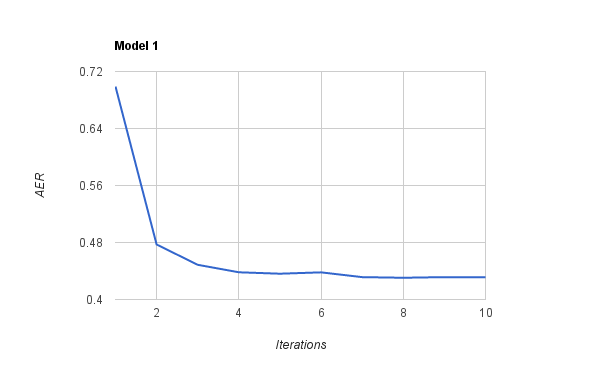
\includegraphics[width=9cm]{model1}
\centering
\caption{Model 1 - AER and Iterations}
\label{figure:model1aer}
\end{figure}

\subsubsection{Error Analysis}

Model 1 produces much more reasonable alignments than PMI.  One of the most obvious
weaknesses that remains is alignments with repeated source words.  Again, because of
the way \texttt{argMax} resolves ties, all repeated source words will align with the
same target word.  This can make it appear that a sentence with three commas in French,
will only have a single comma in English.  In the absence of repeated words (or 
interchangeable words), the model seems to cope well with word order differences.  It appears
more common to align too many words to a word, rather than completely wrong alignments.

There is some garbage collection appearing, with the abbreviation "Mr." aligning
to the period.  Both "M." and "Monsieur" appear in the same sentence, so it's possible
that the probability of aligning "Mr." with french translations is relatively spread out,
while the period appears in most every sentence that "Mr." does.


\subsection{IBM Model 2 Aligner}

The \texttt{IBMModel2Aligner} code is very similar to the 
IBM Model 1 code, with the main differences being an updated alignment probability
function to include distortions, as well as running IBM Model 1 first and using
the resulting $ t $ values to initialize Model 2.  

Again, most of the complexity is pushed into
the \texttt{Model2ExpectationMaximizer} helper.  The helper re-uses the Model 1
EM code, updating the probabilities and counts to include distortions.  I implemented
a method \texttt{getQKey} to manage building keys for the $ q $ probabilities, 
to make it simpler to maintain a consistent index order. 

The \texttt{Model2ExpectationMaximizer} is initialized with $ t(f_i|e_j) $ 
from running the \texttt{Model1ExpectationMaximizer}.  $ q(j|i,l,m) $ is 
initialized uniformly.
During each iteration of my algorithm, I update the counts 
$ C(f_i|e_j) $ and $ C(f|i,l,m) $
by adding $ \delta(k, i, j) $ to each, where 
$ \delta(k, i, j) = \frac{q(j|i,l_k,m_k)t(f_i^k|e_j^k)}{\sum_{j=0}^{l_k}q(j|i,l_k,m_k)t(f_i^k|e_j^k)} $ 
for every source-target word pair in each sentence pair $ k $ (algorithm is Collins Figure 2).
As in Model 1, I calculate the divisor first, outside of the loop.
At the end of each iteration, I normalize both counts.

I run my algorithm for 10 iterations, because as can be seen in Table \ref{table:model2aer}
and Figure \ref{figure:model2aer} the rate of improvement of the AER is fairly flat at that
point.

To calculate alignments after the model is trained, I used 
$ a_i = \argmax_{j\in{0..l}} (q(j|i,l,m) \times t(f_i|e_j)) $.

\subsubsection{Error Analysis}

Model 2 offers subtle improvements over Model 1, but nothing nearly as dramatic as the move
from PMI to Model 1.  Model 2 is definitely still experiencing some garbage collection,
where, for example, many function words align to the English word ruling, but none with the
French word decision.  It definitely still appears that there's a tendency for too many
words to align with a single word.

The addition of distortion probabilities appears to have helped with some of the multiple
alignments, and it appears that most of the duplicate words now align to a word relatively
close to them.  It would be interesting to weight the distortion and translation probabilities,
to see what kind of impact could be had by tuning their relative importance.  Examining the 
Hindi alignments seems to suggest that increasing the importance of the distortion
probabilities could result in better alignments, since many of the missed alignments are pretty
far from where they'd be expected to fall on the diagonal.

Between Model 1 and Model 2, the precision increased from 0.5183 to 0.5758, 
and the recall from 0.6746 to 0.7219.  This relatively modest increase seems to mirror what
I have observed intuitively, the alignments are marginally better, but when they're incorrect,
the issues are very similar to Model 1.

\begin{table}
  \begin{center}
    \begin{tabular}{ l l }
      \hline
      Iteration & AER \\
      \hline
        1  & 0.4607 \\
        2  & 0.3960 \\
        3  & 0.3837 \\
        4  & 0.3775 \\
        5  & 0.3851 \\
        6  & 0.3869 \\
        7  & 0.3841 \\
        8  & 0.3803 \\
        9  & 0.3803 \\
        10 & 0.3775 \\
      \hline
    \end{tabular}
  \end{center}
  \caption{Model 2 AER}
  \label{table:model2aer}
\end{table}

\begin{figure}[t]
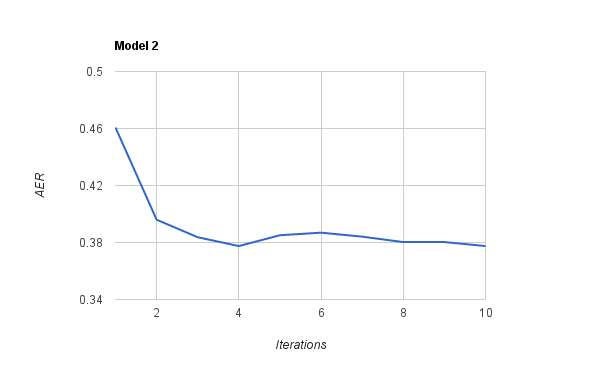
\includegraphics[width=9cm]{model2}
\centering
\caption{Model 2 - AER and Iterations}
\label{figure:model2aer}
\end{figure}

\section{Part 2 - Phrasal Feature}
 
The feature that I implemented added indicators using parts of speech data
extracted from the source and target phrases using CoreNLP.  The total number of weights
learned increased from 10 in the baseline to 6,065.  My measured Phrasal baseline was 
15.4059, and I measured an increase to 15.7609, a difference of 0.355, over 50 runs.

My belief was that some of the target phrases weren't really grammatical, so I thought that
by comparing parts of speech in the source and target, and learning weights for parts of 
speech in the target, the system would be able to generalize a little more about
English sentence structure.

\subsection{Features}

\subsubsection{Bias}

I added a simple indicator bias feature to each rule regardless of source or target phrase,
to act as a constant.  The system learned a weight of $ -0.0572 $ for this feature.  I expected
the bias to be negative, to counteract the weights that I believed would be learned from
parts-of-speech co-occurrences.

\subsection{Target Parts of Speech}

I added unigram, bigram, and trigram part of speech indicator features over the target phrase.
That expectation was that the system could learn in general which English parts of speech
work well together.

For example:

\begin{verbatim}
TARGET_POS_TRIGRAM:IN:NNS:IN
\end{verbatim}

\subsubsection{Part of Speech Co-Occurrence}

I created an indicator feature pairing every part of speech in the source
with every part of speech in the target.  The part of speech tags for
English and French aren't consistent, so this kind of approximates matching
nouns to nouns, for example.

For example:

\begin{verbatim}
POS_CO_OCCUR:JJ:ADJ
\end{verbatim}

\subsubsection{Part of Speech Change}

This indicator feature outputs sorted part of speech tag sets for both the source
 and target phrases.  I decided to sort the tags and put them in sets instead of
 displaying the tags in the order they appeared to avoid over-fitting.

For example: 

\begin{verbatim}
POS_CHANGE:DT|IN|VBZ:CLS|DET|ET|P|V
\end{verbatim}

\subsection{Output Impact}

A few examples are highlighted in Table 5
and Table 6 - in general, where there is improvement,
the sentence tends to follow more common English-language
patterns.

\begin{table}
  \begin{center}
    \begin{tabular}{ l }
      \hline
        \textbf{With Feature} \\
      \hline
        the gdp of germany has a anticipated growth \\ 
        0.5 \% , that of france 0.4 \% . \\
      \hline
        they have won 1:0 in montenegro and\\
        celebrating the qualification for 200 million\\
      \hline
        in the czech republic , only 23 \% of families\\
        of my students eat at the same time .\\
      \hline
        they are not really mistakes , but the expression\\
        of an incomprehensible laziness on the part of the\\
         developers .\\
      \hline
    \end{tabular}
  \end{center}
  \caption{With Feature Translations}
\end{table}

\begin{table}
  \begin{center}
    \begin{tabular}{ l }
      \hline
        \textbf{Baseline} \\
      \hline
        the germany 's gdp growth expected 0.5 \% ,\\
        that of france of 0.4 \% .\\
      \hline
        they have won in montenegro 1:0 and celebrating\\
        qualification for 200 million\\
      \hline
        in the czech republic , only 23 \% of families\\
        of pupils my eat at the same time .\\
      \hline
        they are not really mistakes , but the expression\\
        of an laziness incomprehensible on the part of the\\
        developers .\\
      \hline
    \end{tabular}
  \end{center}
  \caption{Baseline Translations}
\end{table}

\subsection{Error Analysis}

In evaluating, sometimes it appeared that parts of speech matching had won-out
over "better" phrases that were previously selected, probably because they
aren't very common.  On the other hand, it appeared that more natural phrases
were selected overall, probably preferring grammatically correct uncommon phrases.

I believe the biggest room for improvement would be adding a featurizer that ran
over the full or partial target sequence, creating parts of speech trigrams there
as well.  Examining the likelihood of transitions between phrases seems like it would
be pretty fertile ground.

% include your own bib file like this:
%\bibliographystyle{acl}
%\bibliography{acl2015}

\begin{thebibliography}{}

\bibitem[\protect\citename{Manning}2014]{Manning:14}
Manning, Christopher D. and  Surdeanu, Mihai  and  Bauer, John  and  Finkel, Jenny  and  Bethard, Steven J. and  McClosky, David.
\newblock 2014.
\newblock {The {Stanford} {CoreNLP} Natural Language Processing Toolkit}.
\newblock {\em Proceedings of 52nd Annual Meeting of the Association for Computational Linguistics: System Demonstrations},
\newblock pp. 55--60.

\end{thebibliography}

\end{document}
